\documentclass[12pt]{article}
\usepackage[utf8]{inputenc}
\usepackage[margin=1in]{geometry}
\usepackage{amsmath}
\usepackage{graphicx}
\usepackage{enumerate}
\graphicspath{ {./images/} }

\author{Neelu Saraswatibhatla (srns2)}
\title{Operating Systems Supervision 3}
\date{\vspace{-5ex}}

\begin{document}

\maketitle

\section{Example Sheet 4}

\begin{enumerate}
    \item The basic access control scheme is to have read, write, and execute access to each file. More advanced access control policies are implemented by allowing these permissions to be set by user, group, and world.
    \item \begin{enumerate}
        \item As seen in the diagram below, the filesystem contains a boot block and one or more partitions. Each partition has a superblock, an inode table, and data blocks. The boot block contains the location of each filesystem (partition). The superblock contains the number of blocks and free blocks in the filesystem and other bookkeeping information. Free inodes and blocks are located together with allocated ones, and a list is kept of the free ones.\\
        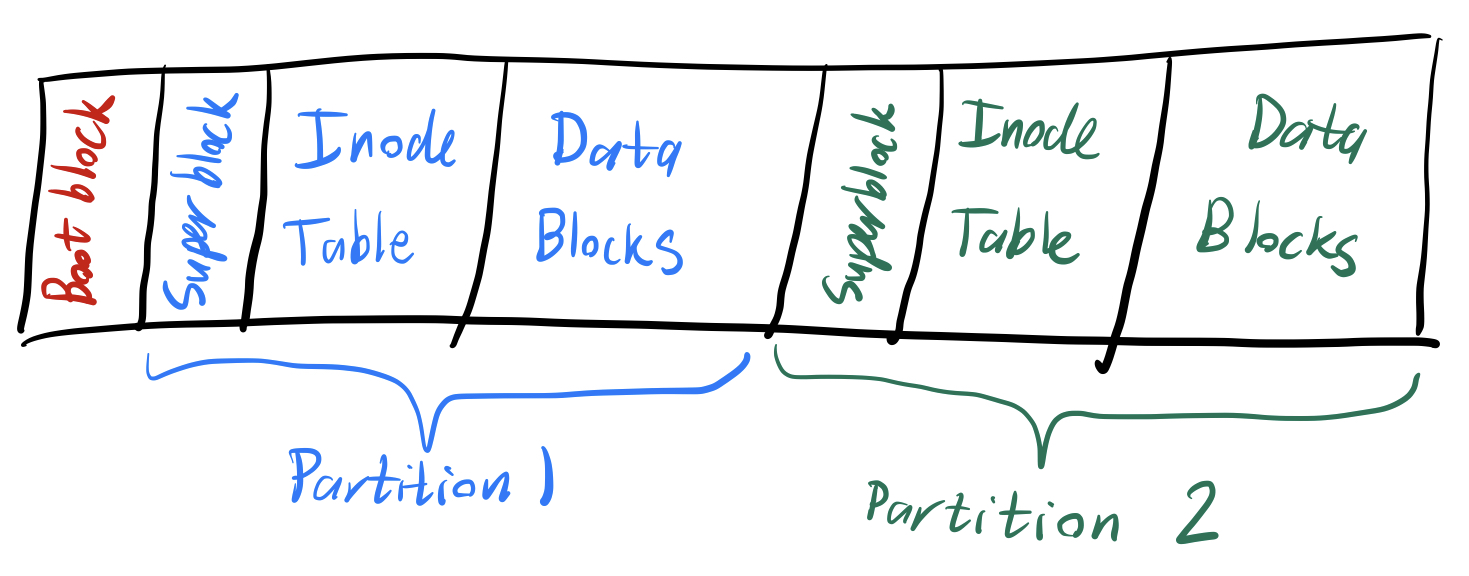
\includegraphics[scale=0.25]{2a.jpg}
        \item An inode contains various things \begin{itemize}
            \item Bookkeeping information such as type, size, etc. It is important to note that the inode does NOT contain the file name or permissions, as these are stored in the directory rather than in the inode.
            \item 12 direct blocks which point directly to data.
            \item A single indirect block which points to 512 direct blocks, each of which point to data.
            \item A double indirect block which points to 512 single indirect blocks.
            \item A triple indirect block which points to 512 double indirect blocks.
        \end{itemize}
        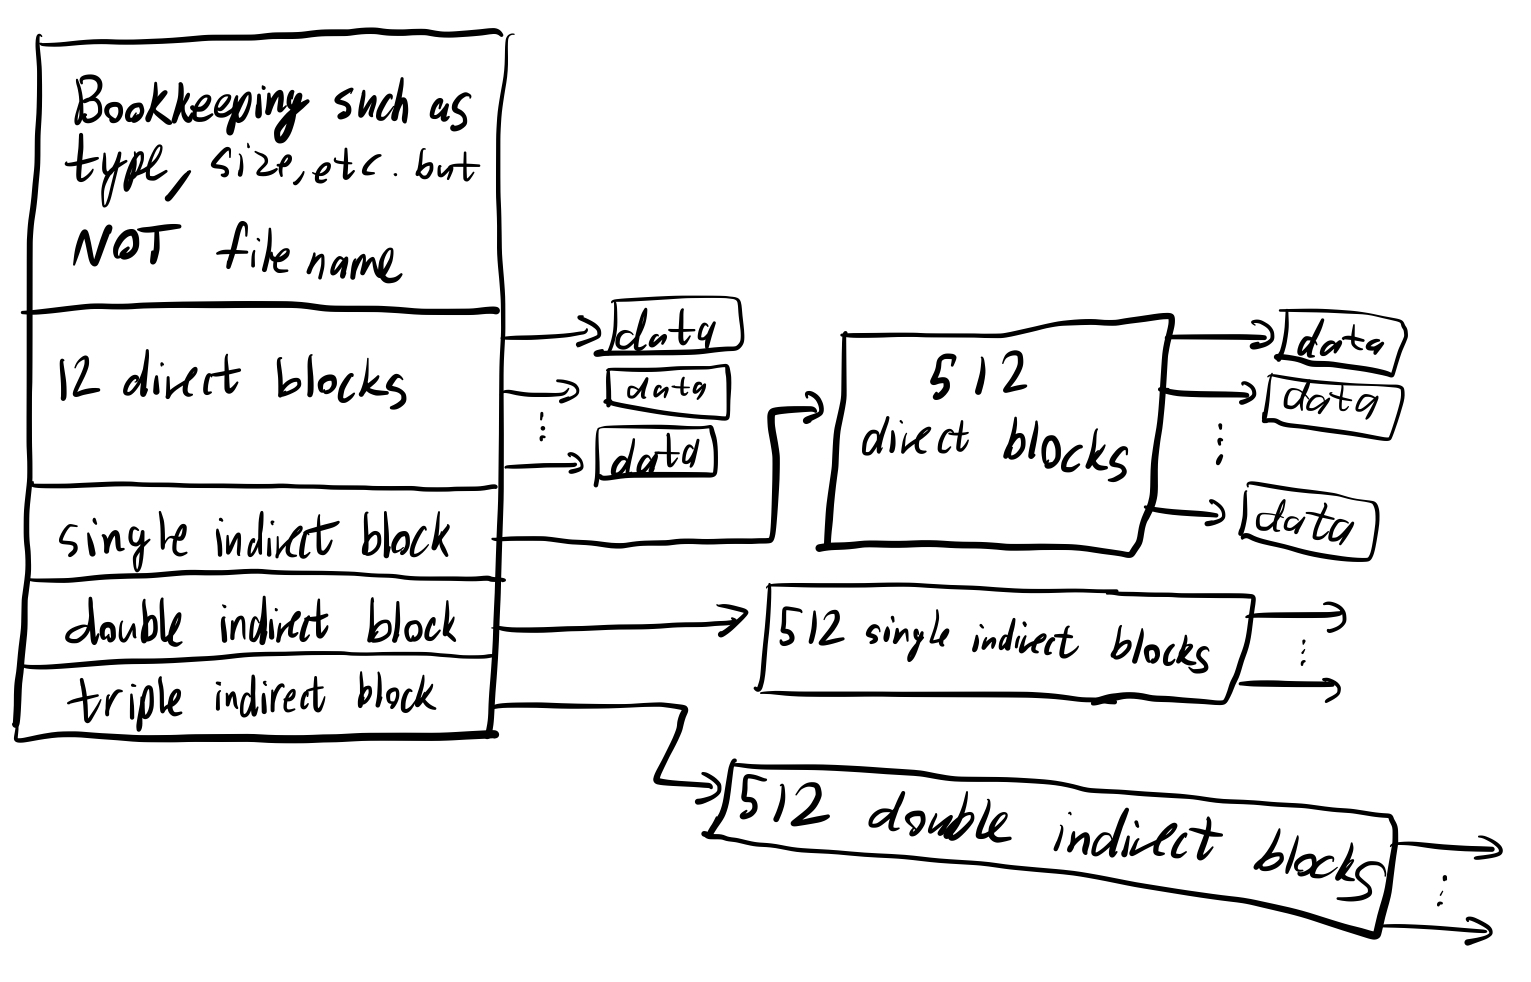
\includegraphics[scale=0.25]{2b.jpg}
        \item \begin{itemize}
            \item 1 triple indirect block $=>$ 512 double indirect blocks $=>$ 512 + 1 = 513 double indirect blocks in total
            \item 513 double indirect blocks $=>$ 513 * 512 = 262656 single indirect blocks $=>$ 262656 + 1 = 262657 single indirect blocks in total
            \item 262657 single indirect blocks $=>$ 262657 * 512 = 134480384 direct blocks $=>$ 134480384 + 12 = 134480396 direct blocks in total
            \item 134480396 direct blocks $\times$ 512 bytes per block $\approx$ 64.1 GB 
        \end{itemize}
        
        

    \end{enumerate}
\end{enumerate}

\end{document}
